\documentclass[../TST.tex]{subfiles}
\begin{document}
\begin{pproblem}
A parallel beam of monochromatic light (wavelength $\lambda=\qty{500}{nm}$) is normally incident on a diffraction grating. The period of the grating is $d\gg \lambda$. A convex lens of focal length $f=\qty{1}{m}$ is placed parallel to the grating. A diffraction pattern is then observed on a screen in the focal plane of the lens. We now rotate the diffraction grating at an angle $\alpha$ with respect to an axis parallel to the slits. The new fourth order maximum is now observed where the fifth order maximum originally was.
\begin{subpart}
	\item Find the angle $\alpha$. \score{1.0}
	\item Given that the fifth order maximum has shifted by $\Delta l=\qty{12.5}{mm}$ along the screen due to the rotation, find the period of the grating $d$ in micrometres. \score{1.0}
	\item The screen is $L=\qty{20}{cm}$ wide and positioned symmetrically with respect to the optical axis. Find the number of maxima $N$ that will be observed on the screen after the rotation. \score{1.0}
\end{subpart}
\end{pproblem}

\ifprob \else
	\begin{solution} (a) In the initial setup, all rays that diffract at an angle $\theta$ form a parallel beam which is focused into a single point on the screen (because the screen is in the focal plane). Any two rays from adjacent slits acquire an optical path difference of $d\sin{\theta}$ at the grating. Since there are many such pairs, the only way to get a maximum on the screen is for all rays to stay in phase, i.e.\,$d\sin{\theta}=n\lambda$ for integer $n$. For a given $n$, we call this the $n$-th order maximum.
\begin{figure}[H]
	\begin{minipage}[b]{0.5\textwidth}
    \centering
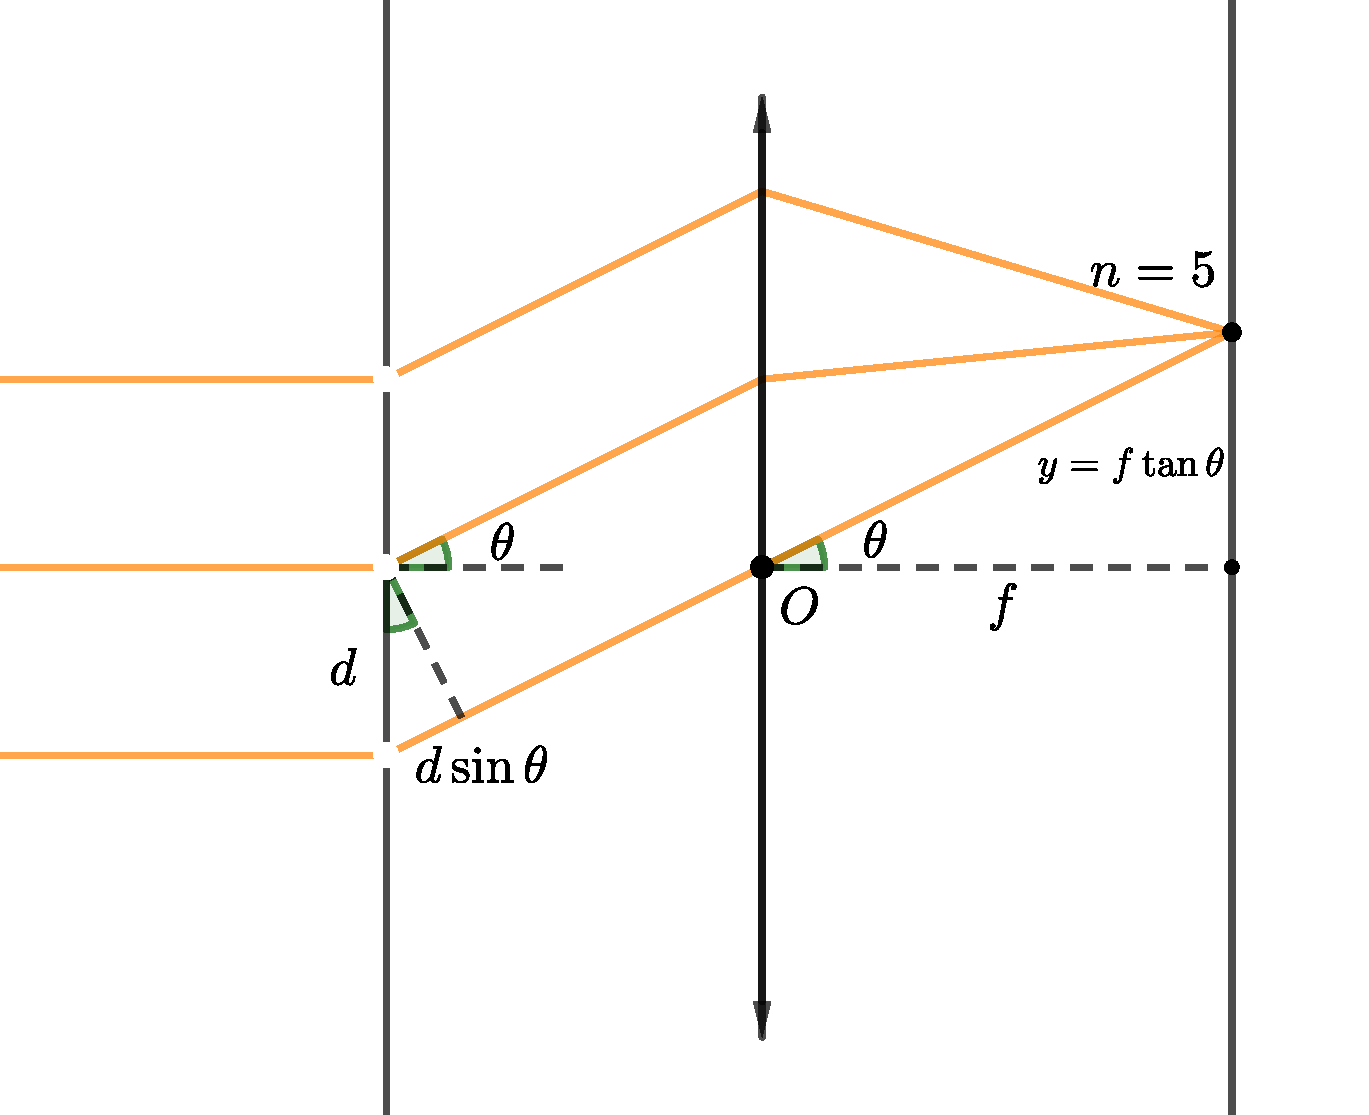
\includegraphics[width=\textwidth]{fig/a2011_s61.pdf}
    % \caption*{}
	\end{minipage}\hfill
	\begin{minipage}[b]{0.5\textwidth}
		\centering
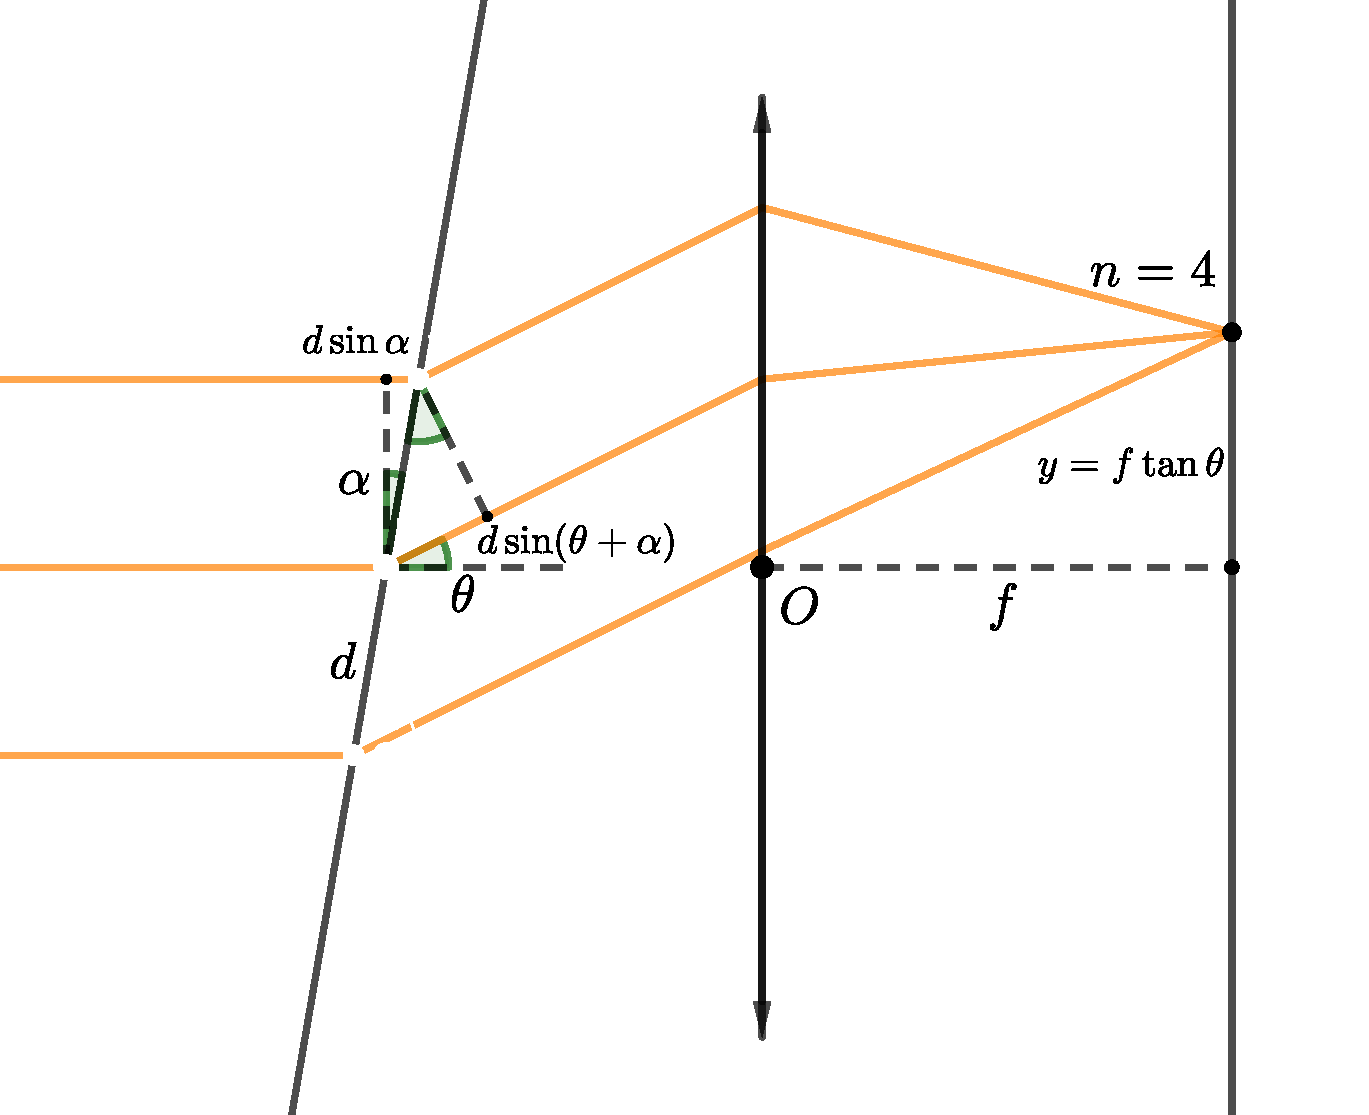
\includegraphics[width=\textwidth]{fig/a2011_s62.pdf}
    % \caption*{}
	\end{minipage}
\end{figure}
	After we rotate the grating by an angle $\alpha$, the optical path difference for the beam at an angle $\theta$ will change to $d(\sin{(\theta+\alpha)}-\sin{\alpha})$. As per the problem statement, for some angle $\theta_5$ we have
\begin{align*}
	&d\sin{\theta_5}=5\lambda,\\
	&d(\sin{(\theta_5+\alpha)}-\sin{\alpha})=4\lambda.
\end{align*}
Since $d\gg\lambda$, the angle $\theta_5$ is expected to be very small. The same cannot be said for $\alpha$, but we are still allowed to approximate $\sin{\theta_5+\alpha}\approx \sin{\alpha}+\theta_5\cos{\alpha}$. Thus
\begin{align*}
	&d{\theta_5}=5\lambda,\\
	&d\theta_5\cos{\alpha}=4\lambda.
\end{align*}
We divide these to find $\cos{\alpha}=4/5$, or $\boxed{\alpha=\ang{36.9}}$. For an exact value of $\alpha$, we'd also need the data from (b). Working out a system of three equations numerically, we could obtain $\alpha=\ang{35.5}$. Evidently our approximate value for $\alpha$ isn't far from the exact answer. \\

(b) Let the new direction of the fifth order maximum correspond to an angle $\theta_5'$. Then,
\begin{equation*}
	\sin{(\theta_5'+\alpha)}-\sin{\alpha}=\sin{\theta_5}=\frac{5\lambda}{d}.
\end{equation*}
Since $\lambda/d$ is small, the difference between $\sin{(\theta_5'+\alpha)}$ and $\sin{\alpha}$ is also small, meaning $\theta_5'$ is a small angle too. We can then use $\sin{(\theta_5'+\alpha)}\approx\sin{\alpha}+\theta_5'\cos{\alpha}$ to get $\theta_5'\cos{\alpha}=\theta_5$, or $\theta_5'=\frac{5}{4}\theta_5$. From the problem statement we gather that
\begin{equation*}
\Delta l = f(\tan\theta_5'-\tan\theta_5) \approx f(\theta_5'-\theta_5)
,
\end{equation*}
which implies $\Delta l=\frac{1}{4}f\theta_5$. However, we also have $\theta_5=\frac{5\lambda}{d}$, so
\begin{equation*}
	\boxed{d=\frac{5\lambda f}{4\Delta l}=\qty{50}{\micro m}.}
\end{equation*}
(c) Only the beams travelling at less than a critical angle $\theta_\mathrm{lim}$ will get focused on the screen. Tracking the rays passing through the centre of the lens, we find
\begin{equation*}
	\tan{\theta_\mathrm{lim}}=\frac{L/2}{f} \quad\Rightarrow\quad \theta_\mathrm{lim}=\ang{5.7}
.
\end{equation*}

After the rotation, angles $\theta_n$ corresponding to maxima obey
\begin{equation*}
	\sin{(\theta_n+\alpha)-\sin{\alpha}}=\frac{n\lambda}{d}
.
\end{equation*}
The function on the left hand side increases with $\theta_n$, which may vary between $-\theta_\mathrm{lim}$ and $+\theta_\mathrm{lim}$. Substituting these limits for $\theta$, we find $n=-8.3$ and $n=7.6$, respectively. This means that the maxima which fit on the screen start from $n=-8$ and end at $n=7$. This is a total of $\boxed{N=16}$ maxima. The number is still the same if we work with the exact values for $\alpha$ and $d$.

\end{solution}
\fi

\end{document}
